\subsubsection{Scattering Model}
\label{scatter}
Scatter is the physical process where incident radiation is absorbed and reflected back towards the atmosphere. To this end a scattering model is used. This scattering model is a way to construct a \ac{BRDF}. A \ac{BRDF} is a distribution of the incident light over the hemisphere \cite[pages 47-49]{rees}. An example is shown in figure \ref{fig:scatter}, page \pageref{fig:scatter}.\\\\
The most basic example of a \ac{BRDF} is the Lambertian model \cite[pages 49-50]{rees}. This model assumes a homogeneous perfectly rough surface, causing a homogeneous scattering distribution. Apart from the index of refraction of the air, the incident radiation vector and the exittant radiation vector (which are all known), use of Snell's law is needed to find Fresnel's coefficients, thereby requiring the index of refraction of the ground.

A modification that can be made to take into account the tendency of surfaces to scatter more in the direction of the surface normal, is called the Minnaert model \cite[page 50]{rees}. It causes a more elliptical \ac{BRDF}. It depends on the Minnaert parameter $\kappa$.

Another important modification is the Henyey-Greenstein term. It accounts for the tendency of surfaces to back- or forwardscatter \cite[page 51]{rees}. This rotates and deforms the elliptical \ac{BRDF} obtained from the Minnaert model. The Henyey-Greenstein term is parameterized by $\Theta$. The final result is shown in figure \ref{fig:scatter}, page \pageref{fig:scatter}.\\\\
This is the scattering model used in the program. Because there is no data from which all three parameters can be accurately determined, a coefficient map was made up. It does not matter much what the precise form of the \ac{BRDF} used in the simulation is, so long as it can be retrieved.

With the help of the formulae from \cite[pages 43-51]{rees}, the incidence vector can be taken and the number of photons radiated in a specific direction can be calculated. Note that the program does not integrate over part of the sphere: because the angle of the cone is very small, the \ac{BRDF} is assumed to be constant over the cone. The error induced here is worth avoiding the computationally expensive integration.


\begin{figure}[ht!]
\centering
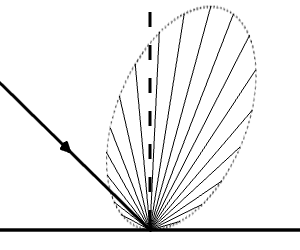
\includegraphics[width=0.4\textwidth]{chapters/img/scatter.png}
\caption{Example of a \ac{BRDF}}
\label{fig:scatter}
\end{figure}